\chapter{Две древнеримские байки}

Щас я расскажу вам две древнеримские байки, чтоб вы лучше понимали античных латинов. Они очень поучительные, и просто пропитаны республиканским колоритом до предела. Как говорится: "такое мог сотворить только наш, римский человек, варвар бы до этого не додумался".
\section{Гай Муций Сцеволла}

Дело было так. 509 год, ещё только набирающая силы Римская республика ведет борьбу за место под солнцем. Борьба идет с переменным успехом. Вот и в этот раз чет пошло не так, и этруски во главе со своим царем Порсеной разбили римлян и осадили Город. И вот сидят латины в осаде, и думают чего им делать.


Хитрый план придумал Гай Муций. Он решил переплыть Тибр, проникнуть в лагерь Порсены, ворваться в его шатер и убить царя этрусков, затыкав его кинжалом. После чего, собственно, переплыл, проник, ворвался и убил, только не Порсену, а его казначея. Тот был просто одет богаче, вот пацан мишени и перепутал. Ну, его, естественно, схватили, и доставили к царю на допрос. Где царь стал жаловаться на то, что обезумевшие римляне уже от отчаяния посылают каких-то детей его убить. Гай на это спросил "ты думаешь что знаешь что такое безумие?", и засунул свою правую руку в пылающую жаровню, прожарив кисть до хрустящей корочки. И пока рука прогорала - пояснил царю что им нет равных в доблести, и их таких 300 человек, поклявшихся убить Порсену любой ценой. Муций промахнулся, поэтому его теперь можно казнить, но осталось ещё 299 ассасинов. И возможно они уже сейчас переплывают и пробираются, чтобы перетыкать вообще всех мужиков в лагере, похожих на царя. После этого Порсена попросил вытащить то что осталось от руки из огня, дал Гаю богатые дары, и срочно заслал его в Рим с посольством, заключил мир, взял выкуп и поспешил уйти обратно домой, подальше от этого поехавшего народа.


Так один юноша спас Рим. Латины высказали Гаю респект за столь выдающуюся доблесть, поставили в его честь колонну на форуме и дали почетный когномен "Сцеволла", тоесть "Левша". 
\begin{figure}[h!tb]
	\centering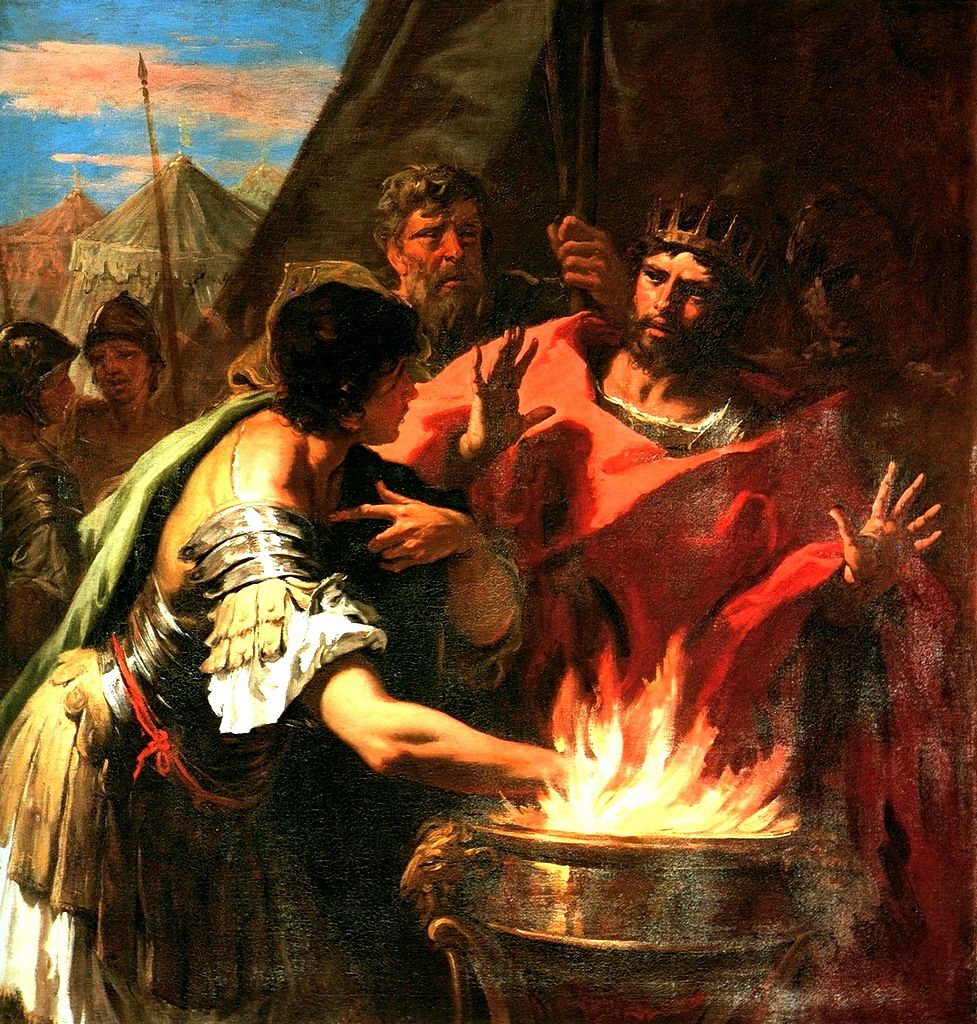
\includegraphics[scale=0.4]{Two_coolstories/1602147758127056135.png}
	\label{fig:coolst1} % Unique label used for referencing the figure in-text
	%\addcontentsline{toc}{figure}{Figure \ref{fig:placeholder}} % Uncomment to add the figure to the table of contents
	\caption{"Я засуну руку в жаровню и пока она горит — не торопясь поясню что тебе пиздец, царь", говорит Гай Муций.	}
\end{figure}

\section{История вторая. Марк Курций}

Если в предыдущей истории мы ещё можем углядеть некие намеки на хитрый план, хоть доблесть и превалирует, то байка про Курция это доблесть в чистом виде. Я бы даже сказал что эт дистиллированная доблесть. А дело было так.


362 год, Рим уже набирает силу и воюет почти каждый год со всеми подряд. Обидных осад больше не случается, скорее наоборот, уже Рим харасит всех своих соседушек. И вот, в один погожий денек случается следующая оказия: после землетрясения прямо на Форуме в земле открывается глубокая трещина. Знак очень нехороший, поэтому римляне на скорую руку пытаются засыпать её всяким говном, но у них ничего не получается. Окей, тогда зовут оракула и спрашивают чойта значит и что делать. Оракул совещается с богами и говорит что боги разгневаны. И римляне должны принести жертву: скинуть в трещину самое ценное что есть в Городе. А иначе ужас-пиздец неминуемый. Все начинают спорить про то, что же в городе самое ценное, но никак не могут прийти к консенсусу. А скидывать туда всё подряд - стремно. Ну и, в общем, пока все совещаются, на форум выезжает наш герой, Марк Курций, в полном боевом облачении и на коне. И говорит: "самое ценное что есть в городе это доблесть и слава. А так как я тут самый охуенный, доблестный и славный, то значит так тому и быть". После чего просто берет и прыгает в трещину прям на коне. И трещина немедленно закрывается - боги приняли жертву. После чего, естественно, римляне говорят "малаца" и называют в честь Курция озеро неподалеку.


Мораль тут следующая. Можно сказать что Сцевола таким макаром боролся за жизнь и умудрился в безвыходной для себя ситуации переиграть царя этрусков и выйти через вход. Он же, в конце концов, не просто выжил, но ещё и достиг цели. Можно также сказать что Курций нажрался как свинья и по пьяни свалился в пропасть, а потом про него уже анекдотов всяких насочиняли. Более того, скорее всего так и есть, томушта оба персонажа легендарные и пруфов нам не завезли. Но тут важно то, что римляне-то и вправду верили что так оно и было. И это чет вроде детских сказок для маленьких латинов, которые неиллюзорно формировали их мировоззрения. Тоесть безотносительно реальности самих случаев наверняка целые поколения подростков представляли себе, что "вырасту, засуну руку в жаровню и буду угрожающему Риму царю спокойно говорить что ему пиздец, пока рука обгорает". Или даже "вырасту и как ебанусь в пропасть в полном боевом, провал сразу и закроется, спасу город от неминумой хуйни, перед богами ценой своей жизни отмажу". Ну и, естественно, если поколениями вливать в исходный код такие истории, то вырастет народ, для которого "смерть за Отечество сладка и приятна".


Латинский термин "Virtus" обычно переводится как доблесть, но для самих римлян это было нечто куда большее. Виртус это все добродетели вместе взятые, плюс слава, подвиги, честь и ещё куча всего. По сути, это некий рейтинг очков, в процессе жизни набранных индивидом, и это то, как его видит общество. Виртус ещё и по наследству передается, поэтому чем славнее твоя фамилия, тем у тебя больше виртуса и тем ты более охуенен. И фармится он, собственно, вот такими вот деяниями, дюже героическими и для всеобщей пользы.


Это очень важно для понимания. Фактически, всю жизнь римлянин дрочит на свой виртус и по максимуму его фармит, а также сравнивает с виртусом коллег по палате, и очень расстраивается если у него короче. Поэтому шансы себя проявить он никогда не упускает. Более того, такие шансы он старается всячески искать и не размениваться на бытовуху. И уж тем более тру-римлянин не упустит возможность умереть за Отечество совершив подвиг, и тем самым заработав просто вагон виртуса одним героическим деянием. Так чтобы хватило и на себя и на кучу поколений потомков, а ещё чтобы на форуме колонну поставили или озеро назвали — ведь тогда виртус будет фармиться даже после смерти, этож вообще охуенно. Что, по сравнению со столь радужными перспективами, стоит какая-то человеческая жизнь? Да ничего не стоит.
\begin{figure}[h!tb]
	\centering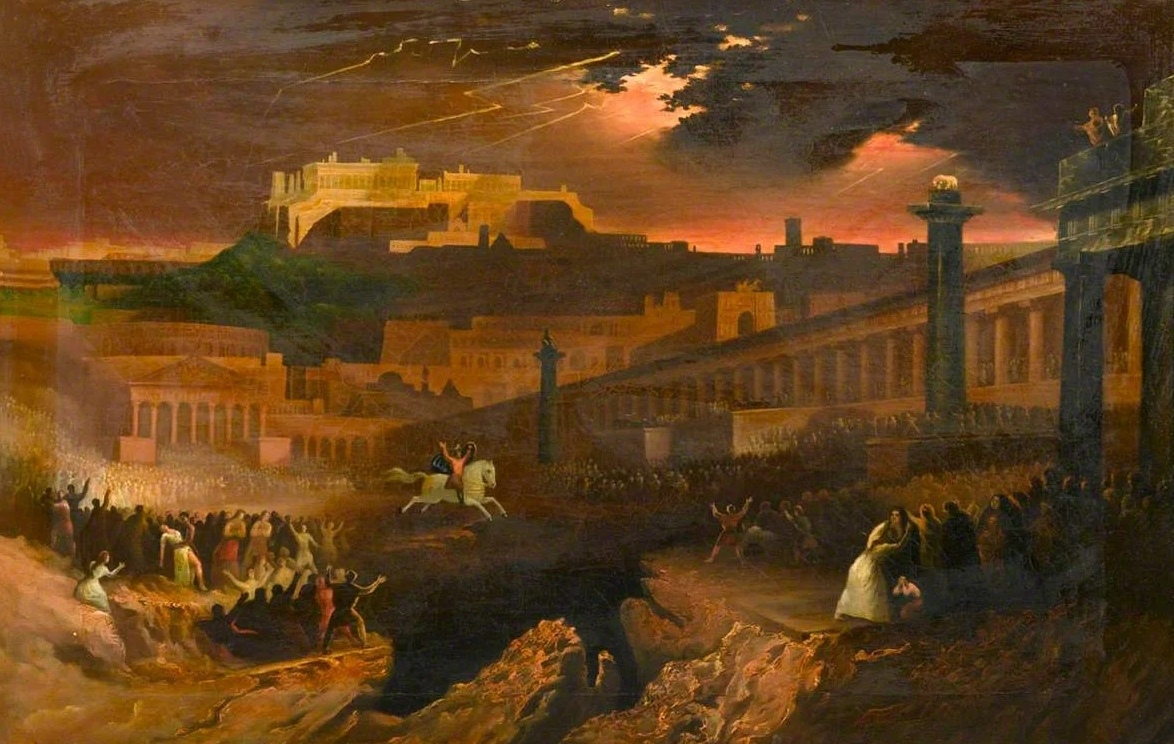
\includegraphics[scale=0.4]{Two_coolstories/1602147873151469527.png}
	\label{fig:coolst2} % Unique label used for referencing the figure in-text
	%\addcontentsline{toc}{figure}{Figure \ref{fig:placeholder}} % Uncomment to add the figure to the table of contents
	\caption{"Я засуну руку в жаровню и пока она горит — не торопясь поясню что тебе пиздец, царь", говорит Гай Муций.	}
\end{figure}

Такие вот дела. Про это не стоит забывать когда мы говорим про античных римлян. Они очень на нас похожи, но, тем не менее, в некоторых моментах кардинально отличаются. У нас, в мире победившего гипериндивидуализма, можно плевать на общество и не испытывать по этому поводу вообще ничего. А римлянин был от общества практически неотделим.


Кстати, именно поэтому одной из самых страшных кар для патриция было изгнание из Города, которое воспринималось хуже смертной казни. Ведь это обнуление всего накопленного виртуса и отсутствие возможности фармить новый. Что делало жизнь бессмысленной и просто невыносимой. И хоть ко временам Поздней Республики это уже, в значительной степени, выветрилось, но вся ранняя история Рима была просто пропитана данным категорическим имперративом.


Короче говоря, латины создали первую и, возможно, последнюю в истории нацию патентованных кармодрочеров с очень специфическим мировоззрением. Да, до них были Платон и Аристотель, а также прочие греки, но там оно носило достаточно локальный характер, не отменяя общего греческого мещанства. Латины же поставили производство подобных личностей на конвейер, и несколько десятков поколений умело воспроизводили. И именно такие вот люди, фармя свой виртус, выебали весь античный мир и сделали Рим великим. 